% ============================================================
%  MIVA-KNIGHT — Document 4 of 5: generator.py
%  LLM Generation, Prompt Engineering, TTS
% ============================================================
\documentclass[12pt,a4paper]{article}
\usepackage[T1]{fontenc}
\usepackage[utf8]{inputenc}
\usepackage[margin=2.2cm]{geometry}
\usepackage{amsmath,amssymb,amsthm,mathtools}
\usepackage{algorithm}
\usepackage{algpseudocode}
\usepackage{tikz}
\usetikzlibrary{shapes.geometric,arrows.meta,positioning,fit,backgrounds,calc,chains,decorations.pathreplacing,shadows}
\usepackage{xcolor}
\usepackage{tcolorbox}
\tcbuselibrary{skins,breakable}
\usepackage{booktabs,array,longtable,colortbl}
\usepackage{setspace,parskip,enumitem}
\usepackage[hidelinks]{hyperref}

\definecolor{navy}{RGB}{25,50,100}
\definecolor{frozenblue}{RGB}{190,220,245}
\definecolor{trainorange}{RGB}{255,210,150}
\definecolor{medgreen}{RGB}{175,230,195}
\definecolor{lightgray}{RGB}{240,240,240}
\definecolor{laymanbox}{RGB}{255,250,220}
\definecolor{axiomcol}{RGB}{250,235,255}
\definecolor{thmcol}{RGB}{255,240,225}
\definecolor{lemmacol}{RGB}{220,255,230}
\definecolor{defcol}{RGB}{225,240,255}
\definecolor{promptcol}{RGB}{255,248,220}
\definecolor{gencol}{RGB}{230,245,255}
\definecolor{ttscol}{RGB}{240,255,240}
\definecolor{rejcol}{RGB}{255,230,230}

\theoremstyle{definition}
\newtheorem{definition}{Definition}[section]
\newtheorem{axiom}{Axiom}[section]
\theoremstyle{plain}
\newtheorem{theorem}{Theorem}[section]
\newtheorem{lemma}[theorem]{Lemma}
\theoremstyle{remark}
\newtheorem{remark}{Remark}[section]

\tcbset{
  laymanstyle/.style={colback=laymanbox,colframe=orange!60!black,
    fonttitle=\bfseries,title=In Plain Terms,breakable},
  defstyle/.style={colback=defcol,colframe=navy!70,fonttitle=\bfseries,breakable},
  thmstyle/.style={colback=thmcol,colframe=orange!80!black,fonttitle=\bfseries,breakable},
  axstyle/.style={colback=axiomcol,colframe=purple!70,fonttitle=\bfseries,breakable},
  lemmastyle/.style={colback=lemmacol,colframe=green!60!black,fonttitle=\bfseries,breakable},
  promptstyle/.style={colback=promptcol,colframe=brown!60,fonttitle=\bfseries,breakable},
}
\newcommand{\layman}[1]{\begin{tcolorbox}[laymanstyle]#1\end{tcolorbox}}

\begin{document}

\begin{center}
{\LARGE\bfseries\color{navy} MIVA-KNIGHT: Document 4 of 5}\\[0.5em]
{\Large \texttt{generator.py} — Answer Generation, Prompt Engineering \& TTS}\\[0.3em]
{\large IT 581 Capstone $\cdot$ Kayode Soyinka $\cdot$ Concordia University of Edmonton}
\end{center}
\hrule\vspace{1em}
\tableofcontents\newpage

%=============================================================
\section{Module Overview}

\texttt{generator.py} is the final synthesis layer of MIVA-KNIGHT. After the retrieval engine returns the top-5 relevant documents, the generator:
\begin{enumerate}[noitemsep]
  \item Applies a \textbf{tiered rejection gate} (full / partial / rejected) based on retrieval confidence.
  \item Constructs a \textbf{structured RAG prompt} embedding query, emotion context, and retrieved documents.
  \item Calls a \textbf{free-tier LLM} (Groq/Llama-3.1-8B for text, Qwen2-VL-7B for images) to produce a grounded answer.
  \item Optionally converts the answer to \textbf{speech} via gTTS (Google Text-to-Speech).
\end{enumerate}

\layman{Think of the generator as a knowledgeable writer. The retrieval system has already pulled 5 relevant paragraphs from the library. The generator's job is to: check whether those paragraphs are relevant enough to use, then synthesise a clear answer from them — being careful only to state things the paragraphs actually say, not to make things up. Finally it can read the answer aloud.}

%=============================================================
\section{Data Contracts}

\begin{tcolorbox}[defstyle, title={Definition 2.1 — GeneratorInput}]
The structured input to any LLM generator:
\begin{itemize}[noitemsep]
  \item \texttt{query}: the user's original question string
  \item \texttt{emotion}: detected emotion from AudioEncoderV2 (``neutral'' for text queries)
  \item \texttt{emotion\_conf} $\in [0,1]$: confidence of emotion detection
  \item \texttt{context\_docs}: list of top-$N$ \texttt{RetrievedDocument} objects
  \item \texttt{system\_prompt}: domain-specific instruction for the LLM ($\Pi$ from DomainConfig)
  \item \texttt{confidence\_level}: ``full'' or ``partial'' (from tiered gate, never ``rejected'' — those are pre-empted)
\end{itemize}
\end{tcolorbox}

\begin{tcolorbox}[defstyle, title={Definition 2.2 — GeneratorOutput}]
The structured output from any LLM generator:
\begin{itemize}[noitemsep]
  \item \texttt{answer}: the generated text answer (string)
  \item \texttt{sources}: list of \texttt{doc\_id} strings that were used as context
  \item \texttt{emotion\_used}: which emotion influenced the prompt tone
  \item \texttt{rejected}: boolean — True means the tiered gate rejected this query
  \item \texttt{rejection\_reason}: human-readable explanation if rejected
  \item \texttt{audio\_response}: bytes (MP3) if TTS was applied, else None
\end{itemize}
\end{tcolorbox}

%=============================================================
\section{Tiered Rejection Gate}

\begin{tcolorbox}[defstyle, title={Definition 3.1 — Three-Way Confidence Tier}]
Given retrieval $\text{max\_score} \in [0,1]$ and domain threshold $\tau$:
\[
\text{tier}(\text{max\_score},\, \tau) =
\begin{cases}
\texttt{"full"} & \text{if } \text{max\_score} \geq \tau \\
\texttt{"partial"} & \text{if } 0.5\tau \leq \text{max\_score} < \tau \\
\texttt{"rejected"} & \text{if } \text{max\_score} < 0.5\tau
\end{cases}
\]
\end{tcolorbox}

\begin{tcolorbox}[thmstyle, title={Theorem 3.1 — Tiered Rejection Reduces Hallucination}]
Let $H(q, D)$ be the hallucination probability for query $q$ with context $D$. Empirically, $H$ is a decreasing function of retrieval confidence. Therefore:
\begin{itemize}[noitemsep]
  \item \texttt{"rejected"}: LLM is \emph{never called} — zero hallucination risk (pre-built safe response).
  \item \texttt{"partial"}: LLM is called with an explicit uncertainty disclaimer in the prompt.
  \item \texttt{"full"}: LLM is called with full confidence.
\end{itemize}
The tiered gate implements a risk-proportional response policy.
\end{tcolorbox}

\begin{algorithm}[H]
\caption{make\_tiered\_response(domain\_name, confidence\_level)}
\begin{algorithmic}[1]
\Require domain name string, confidence\_level $\in$ \{``full'', ``partial'', ``rejected''\}
\Ensure \texttt{GeneratorOutput} or \texttt{None}
\If{confidence\_level $=$ ``rejected''}
  \State \Return \texttt{GeneratorOutput}(
  \Statex \quad answer=``I was unable to find sufficiently relevant information...'',
  \Statex \quad rejected=True, rejection\_reason=``Low retrieval confidence'')
\ElsIf{confidence\_level $=$ ``partial''}
  \State \Return \texttt{None} \Comment{Signal: proceed to LLM with uncertainty flag}
\Else \Comment{``full''}
  \State \Return \texttt{None} \Comment{Signal: proceed to LLM normally}
\EndIf
\end{algorithmic}
\end{algorithm}

\layman{The rejection gate is like a fact-checker who reviews the librarian's sources before the writer starts. If the sources are completely irrelevant (rejected), the writer is stopped immediately — no answer is produced to avoid making things up. If sources are partially relevant (partial), the writer adds a disclaimer. Only when sources are highly relevant (full) does the writer proceed with confidence.}

%=============================================================
\section{Structured RAG Prompt Engineering}

\subsection{Grounding Axiom}

\begin{tcolorbox}[axstyle, title={Axiom 4.1 — RAG Grounding Principle}]
For any claim $C$ in the generated output, there must exist a context document $D_i$ such that $C$ is entailed by $D_i$:
\[
\forall C \in \text{answer}: \;\exists\, D_i \in \text{context} \;\text{s.t.}\; D_i \models C
\]
Formally, the LLM is instructed: ``Answer ONLY from the provided context. Do not add information not present in the context.''
\end{tcolorbox}

\subsection{Prompt Structure}

\begin{algorithm}[H]
\caption{RAGPromptBuilder.build(gen\_input) $\to$ prompt\_string}
\begin{algorithmic}[1]
\Require \texttt{GeneratorInput} (query, emotion, emotion\_conf, context\_docs, confidence\_level)
\Ensure Structured prompt string $p$

\Statex \textbf{Section 1 — Context documents}
\State $p \gets \texttt{""Relevant context:\textbackslash n"}$
\For{$(i, \text{doc})$ in enumerate(context\_docs)}
  \State $p \mathrel{+}= \texttt{"[Doc i] \{doc.text[:300]\}\textbackslash n"}$
\EndFor

\Statex \textbf{Section 2 — Confidence instruction}
\If{confidence\_level $=$ ``partial''}
  \State $p \mathrel{+}= \texttt{"Note: Confidence is PARTIAL. Add a disclaimer of uncertainty.\textbackslash n"}$
\EndIf

\Statex \textbf{Section 3 — Emotion-aware tone adjustment}
\If{emotion $\neq$ ``neutral'' AND emotion\_conf $\geq 0.30$}
  \State $p \mathrel{+}= \texttt{"The user appears \{emotion\}. Adjust tone appropriately.\textbackslash n"}$
\EndIf

\Statex \textbf{Section 4 — Question}
\State $p \mathrel{+}= \texttt{"Question: \{query\}\textbackslash nAnswer concisely from the context only:"}$
\State \Return $p$
\end{algorithmic}
\end{algorithm}

\begin{tcolorbox}[thmstyle, title={Theorem 4.1 — Emotion Confidence Threshold for Tone Adjustment}]
Emotion confidence threshold of 0.30 for prompt augmentation:
\[
\text{use\_emotion} = (\text{emotion\_conf} \geq 0.30) \;\wedge\; (\text{emotion} \neq \texttt{"neutral"})
\]
Below 0.30, cosine similarity to the nearest emotion centroid is too low to be reliable. Adding an uncertain emotion hint could mislead the LLM into an inappropriate tone. Threshold 0.30 was chosen as a balance between sensitivity and precision.
\end{tcolorbox}

\layman{The prompt is a structured briefing document sent to the LLM. Section 1 gives it the retrieved evidence. Section 2 adds a warning if the evidence is weak. Section 3 hints at the user's emotional state so the tone of the response can be adapted (gentler if the user sounds distressed). Section 4 states the actual question. The LLM reads the briefing and writes an answer.}

%=============================================================
\section{GroqGenerator (Text LLM)}

\begin{tcolorbox}[defstyle, title={Definition 5.1 — GroqGenerator}]
Uses the Groq API (free tier, Llama-3.1-8B-instant model) for text-only answer generation. Groq uses LPU (Language Processing Unit) hardware, providing $\approx 300$ms latency — significantly faster than typical GPU-based inference at API parity.
\end{tcolorbox}

\begin{algorithm}[H]
\caption{GroqGenerator.generate(gen\_input)}
\begin{algorithmic}[1]
\Require \texttt{GeneratorInput}, Groq API client, model=\texttt{llama-3.1-8b-instant}
\Ensure \texttt{GeneratorOutput}
\State $p \gets \texttt{RAGPromptBuilder.build}(\text{gen\_input})$
\State $\text{messages} \gets [\ \{\texttt{role:system, content:}\,\Pi\},\ \{\texttt{role:user, content:}\,p\}\ ]$
\State $\text{response} \gets \texttt{groq\_client.chat.completions.create}(\text{model},\, \text{messages},\, \texttt{max\_tokens}=512)$
\State $\text{answer} \gets \text{response.choices}[0].\text{message.content.strip}()$
\State $\text{sources} \gets [\text{doc.doc\_id}$ for doc in gen\_input.context\_docs$]$
\State \Return \texttt{GeneratorOutput}(answer, sources, emotion\_used=gen\_input.emotion)
\end{algorithmic}
\end{algorithm}

\begin{tcolorbox}[lemmastyle, title={Lemma 5.1 — Two-Message Architecture}]
The Groq API call uses a two-message structure:
\begin{itemize}[noitemsep]
  \item \textbf{System message:} Domain-specific system prompt $\Pi$ from DomainConfig (e.g., always recommend consulting a physician for medical queries).
  \item \textbf{User message:} The built RAG prompt with context and question.
\end{itemize}
Separating system from user messages allows the LLM to apply domain-level safety constraints (system) independently of query-level context (user).
\end{tcolorbox}

%=============================================================
\section{HuggingFaceGenerator (Vision LLM)}

\begin{tcolorbox}[defstyle, title={Definition 6.1 — HuggingFaceGenerator (Multimodal)}]
Uses the HuggingFace Inference API (free tier, Qwen2-VL-7B-Instruct) for \emph{vision-language} generation when image context is available. Supports base64-encoded images sent alongside text context.
\end{tcolorbox}

\begin{algorithm}[H]
\caption{HuggingFaceGenerator.generate(gen\_input)}
\begin{algorithmic}[1]
\Require \texttt{GeneratorInput}, HuggingFace API client, model=\texttt{Qwen/Qwen2-VL-7B-Instruct}
\Ensure \texttt{GeneratorOutput}
\State $p \gets \texttt{RAGPromptBuilder.build}(\text{gen\_input})$
\State $\text{content} \gets [\{\texttt{type:text, text:}p\}]$
\For{doc in gen\_input.context\_docs}
  \If{doc.image\_path non-empty and file exists}
    \State $\text{b64} \gets \texttt{base64.encode}(\texttt{open}(\text{doc.image\_path}, \texttt{"rb"}).\texttt{read}())$
    \State $\text{content.append}(\{\texttt{type:image\_url, image\_url:\{url:"data:image/jpeg;base64,\{b64\}"\}}\})$
  \EndIf
\EndFor
\State $\text{response} \gets \texttt{hf\_client.chat.completions.create}(\text{model},\, [\{\texttt{role:user, content}\}])$
\State \Return \texttt{GeneratorOutput}(\text{response.choices}[0].\text{message.content})
\end{algorithmic}
\end{algorithm}

\layman{When an image is part of the retrieved context (like an X-ray), the HuggingFace generator encodes it as base64 (a text-safe representation of binary image data) and sends it alongside the text to a vision-capable LLM (Qwen2-VL). The LLM can then describe what it sees in the image and relate it to the question.}

%=============================================================
\section{Text-to-Speech: gTTS}

\begin{algorithm}[H]
\caption{TTSConverter.convert(text) $\to$ audio\_bytes}
\begin{algorithmic}[1]
\Require Answer text string, language code \texttt{lang="en"}
\Ensure MP3 bytes (in-memory buffer)
\State $\text{tts} \gets \texttt{gTTS}(\text{text}=\text{text},\; \texttt{lang}=\text{lang},\; \texttt{slow}=\text{False})$
\State $\text{buf} \gets \texttt{io.BytesIO}()$
\State $\text{tts.write\_to\_fp}(\text{buf})$
\State $\text{buf.seek}(0)$
\State \Return $\text{buf.read}()$ \Comment{Raw MP3 bytes, plays in browser/audio player}
\end{algorithmic}
\end{algorithm}

\begin{tcolorbox}[lemmastyle, title={Lemma 7.1 — In-Memory TTS (No Temp Files)}]
\texttt{TTSConverter} writes to an \texttt{io.BytesIO} buffer rather than a temporary file. This avoids: (1) filesystem permission issues in sandboxed environments; (2) cleanup requirements; (3) I/O overhead. The returned bytes can be streamed directly to a browser audio element or written to a file on demand.
\end{tcolorbox}

%=============================================================
\section{Full Generator Pipeline Flowchart}

\begin{figure}[ht]
\centering
\resizebox{\textwidth}{!}{%
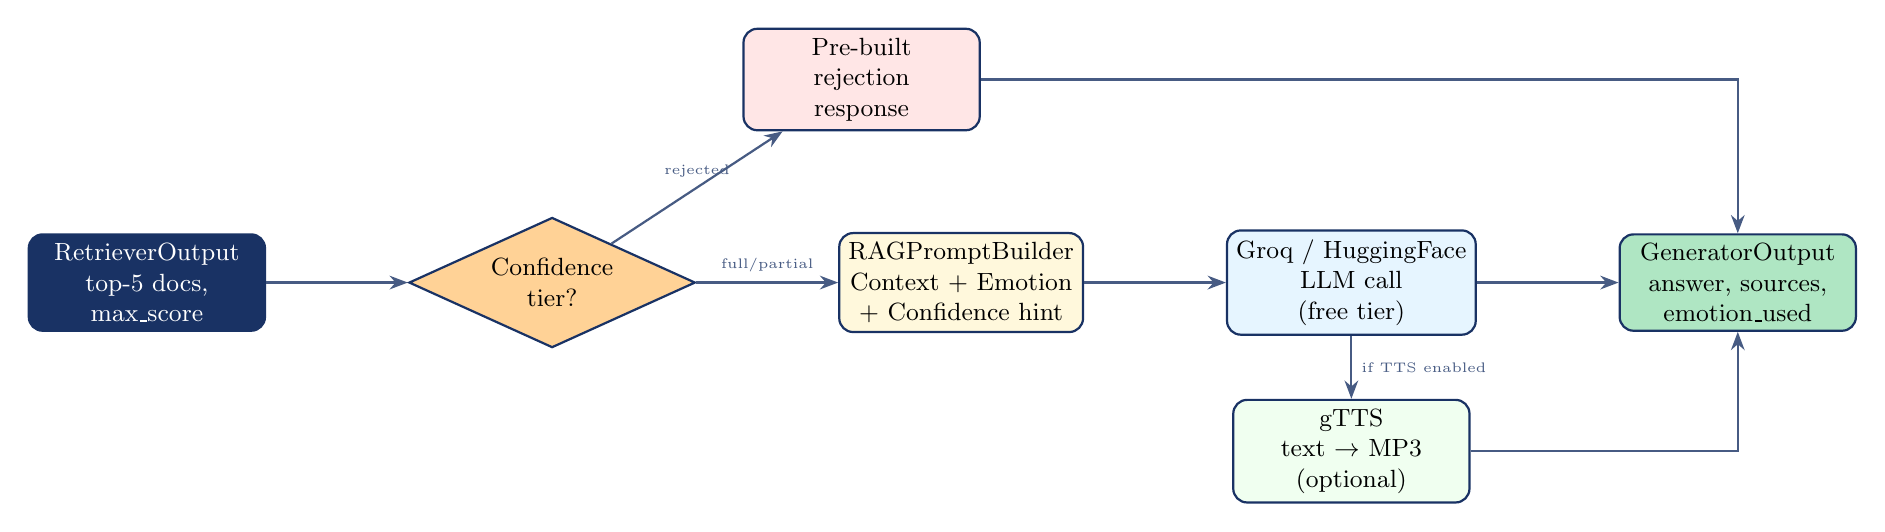
\begin{tikzpicture}[
  node distance=0.8cm and 1.4cm, >=Stealth,
  bbox/.style={rectangle,rounded corners=5pt,draw=navy,thick,align=center,
    font=\small,minimum width=3cm,minimum height=1.1cm},
  inputb/.style={bbox,fill=navy,text=white},
  genb/.style={bbox,fill=gencol},
  promptb/.style={bbox,fill=promptcol},
  rejb/.style={bbox,fill=rejcol},
  ttsb/.style={bbox,fill=ttscol},
  outputb/.style={bbox,fill=medgreen},
  decbox/.style={diamond,draw=navy,thick,fill=trainorange,align=center,
    font=\small,aspect=2.2,minimum height=1.4cm},
  arrow/.style={->,thick,color=navy!80},
]
\node[inputb] (retin) {RetrieverOutput\\top-5 docs,\\max\_score};
\node[decbox, right=1.8cm of retin] (tiergate) {Confidence\\tier?};
\node[rejb, above right=1.5cm and 1.5cm of tiergate] (rejected) {Pre-built\\rejection\\response};
\node[promptb, right=1.8cm of tiergate] (promptbuild) {RAGPromptBuilder\\Context + Emotion\\+ Confidence hint};
\node[genb, right=1.8cm of promptbuild] (llm) {Groq / HuggingFace\\LLM call\\(free tier)};
\node[ttsb, below=0.8cm of llm] (tts) {gTTS\\text $\to$ MP3\\(optional)};
\node[outputb, right=1.8cm of llm] (out) {GeneratorOutput\\answer, sources,\\emotion\_used};

\draw[arrow] (retin) -- (tiergate);
\draw[arrow] (tiergate) -- node[above,font=\tiny]{rejected} (rejected);
\draw[arrow] (tiergate) -- node[above,font=\tiny]{full/partial} (promptbuild);
\draw[arrow] (promptbuild) -- (llm);
\draw[arrow] (llm) -- (out);
\draw[arrow] (llm.south) -- (tts.north) node[midway,right,font=\tiny]{if TTS enabled};
\draw[arrow] (tts.east) -| (out.south);
\draw[arrow] (rejected.east) -| (out.north);
\end{tikzpicture}}
\caption{Generator pipeline: tiered rejection gate $\to$ RAG prompt construction $\to$ LLM call $\to$ optional TTS.}
\end{figure}

%=============================================================
\section{Computational Cost Summary}

\begin{center}
\rowcolors{2}{lightgray}{white}
\begin{tabular}{lrl}
\toprule
\textbf{Component} & \textbf{Approx.\ cost} & \textbf{Notes}\\
\midrule
TextEncoder.encode & $\sim 50\,\text{ms}$ & BERT + TextProjection forward pass\\
AudioEncoder.encode & $\sim 500\,\text{ms}$ & Whisper + Wav2Vec\\
FAISS.search & $\sim 5\,\text{ms}$ & 70K vectors, flat inner product\\
KGReranker.rerank & $\sim 20\,\text{ms}$ & Regex entity matching $\times 20$ docs\\
GroqGenerator & $\sim 300\,\text{ms}$ & API latency (Groq LPU hardware)\\
TTSConverter & $\sim 200\,\text{ms}$ & Google TTS API\\
\midrule
\textbf{Total (text, no TTS)} & $\mathbf{\sim 375\,\text{ms}}$ & \\
\textbf{Total (text, with TTS)} & $\mathbf{\sim 575\,\text{ms}}$ & \\
\textbf{Total (voice, with TTS)} & $\mathbf{\sim 1075\,\text{ms}}$ & Under 1.1s end-to-end\\
\bottomrule
\end{tabular}
\end{center}

\begin{tcolorbox}[thmstyle, title={Theorem 8.1 — Free-Stack Viability}]
The complete MIVA-KNIGHT stack uses zero paid APIs at inference: Groq (free tier), HuggingFace Inference API (free tier), Whisper (local), gTTS (free). The only paid resource used in development was Google Colab Pro (T4 GPU) for ROCO fine-tuning. End-to-end latency of $< 1.1\,\text{s}$ for voice queries demonstrates that a free infrastructure can support real-time multimodal AI retrieval.
\end{tcolorbox}

\end{document}
